\documentclass{article}
\usepackage[utf8]{inputenc}
\usepackage[greek,english]{babel}
\usepackage{alphabeta}
\usepackage{graphicx}
\usepackage{amsmath}
\usepackage{hyperref}
\usepackage{longtable}
\usepackage{geometry}
\usepackage{listings}
\geometry{a4paper, margin=1in}
\usepackage{textgreek}

\title{Αναφορά Ανάλυσης Δεδομένων F1}
\author{Παύλος - Μάριος Γιαννάκος, Σταμάτης Πέτρου}
\date{\today}

\begin{document}

\maketitle

\begin{abstract}
Αυτή η αναφορά παρουσιάζει την εφαρμογή ανάλυσης δεδομένων F1, η οποία αναπτύχθηκε χρησιμοποιώντας τη βιβλιοθήκη Streamlit. Η εφαρμογή επιτρέπει την φόρτωση δεδομένων, την εκτέλεση διερευνητικής ανάλυσης δεδομένων (EDA), την οπτικοποίηση σε δύο διαστάσεις, την ταξινόμηση και την ομαδοποίηση.
\end{abstract}

\section{Εισαγωγή}
Η ανάλυση δεδομένων αποτελεί κρίσιμη διαδικασία για την εξαγωγή χρήσιμων πληροφοριών από μεγάλα σύνολα δεδομένων. Η εφαρμογή αυτή χρησιμοποιεί τις τελευταίες τεχνολογίες στη μηχανική μάθηση και την ανάλυση δεδομένων για να παρέχει μια ολοκληρωμένη λύση ανάλυσης δεδομένων F1.

\section{Τεχνολογίες και Εργαλεία}
\subsection{Βιβλιοθήκες Python}
Η εφαρμογή αξιοποιεί τις παρακάτω βιβλιοθήκες:
\begin{itemize}
    \item \textbf{Streamlit}: Για την ανάπτυξη της διαδραστικής διεπαφής.
    \item \textbf{Pandas}: Για την φόρτωση και επεξεργασία των δεδομένων.
    \item \textbf{NumPy}: Για αριθμητικούς υπολογισμούς.
    \item \textbf{Scikit-learn}: Για την εκτέλεση μοντέλων μηχανικής μάθησης.
    \item \textbf{Matplotlib} και \textbf{Seaborn}: Για την οπτικοποίηση δεδομένων.
    \item \textbf{PlantUML}: Για τη δημιουργία UML διαγραμμάτων.
\end{itemize}

\section{Δυνατότητες Εφαρμογής}
Η εφαρμογή περιλαμβάνει τις ακόλουθες δυνατότητες:

\subsection{Φόρτωση Δεδομένων}
Οι χρήστες μπορούν να φορτώσουν αρχεία δεδομένων σε μορφή CSV ή XLSX. Η εφαρμογή εμφανίζει μια προεπισκόπηση των δεδομένων και διαχωρίζει τα χαρακτηριστικά από τις ετικέτες.

\subsection{Διερευνητική Ανάλυση Δεδομένων (EDA)}
\begin{itemize}
    \item \textbf{Περιγραφή Δεδομένων}: Παρουσιάζει στατιστικά στοιχεία για τα δεδομένα.
    \item \textbf{Μητρώο Συνοσχετισμών}: Εμφανίζει ένα heatmap των συσχετίσεων μεταξύ των χαρακτηριστικών.
    \item \textbf{Pairplot}: Δημιουργεί διαγράμματα ζευγών για να αναδείξει τις σχέσεις μεταξύ των χαρακτηριστικών.
\end{itemize}

\begin{figure}[h!]
    \centering
    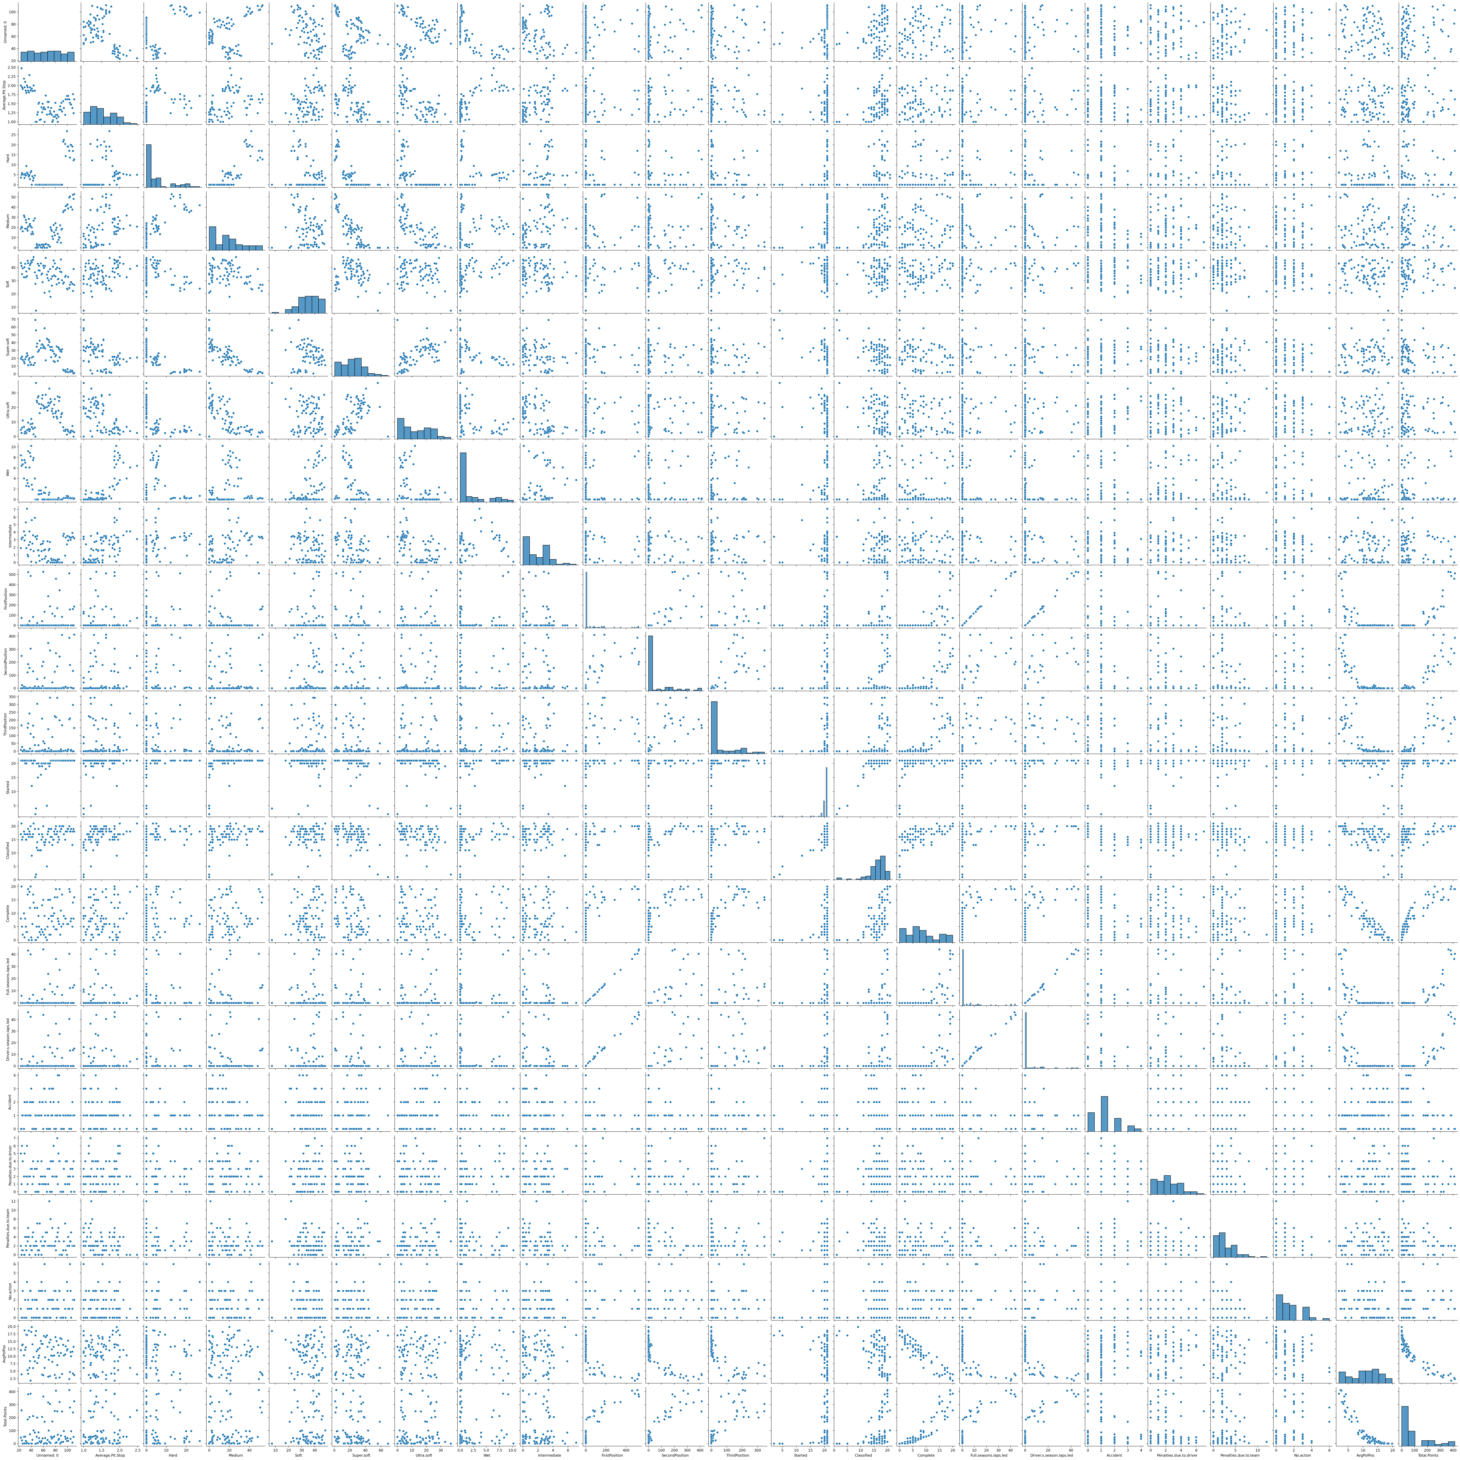
\includegraphics[width=\textwidth]{Pairplot.png}
    \caption{Pairplot}
    \label{fig:pairplot}
\end{figure}

\subsection{Οπτικοποίηση σε Δύο Διαστάσεις}
Η εφαρμογή παρέχει δύο μεθόδους οπτικοποίησης:
\begin{itemize}
    \item \textbf{PCA (Ανάλυση Κύριων Συνιστωσών)}: Μειώνει τη διάσταση των δεδομένων σε δύο κύριες συνιστώσες και τα οπτικοποιεί.
    \item \textbf{t-SNE (t-Distributed Stochastic Neighbor Embedding)}: Προβάλλει τα δεδομένα σε δύο διαστάσεις χρησιμοποιώντας τον αλγόριθμο t-SNE.
\end{itemize}

\begin{figure}[h!]
    \centering
    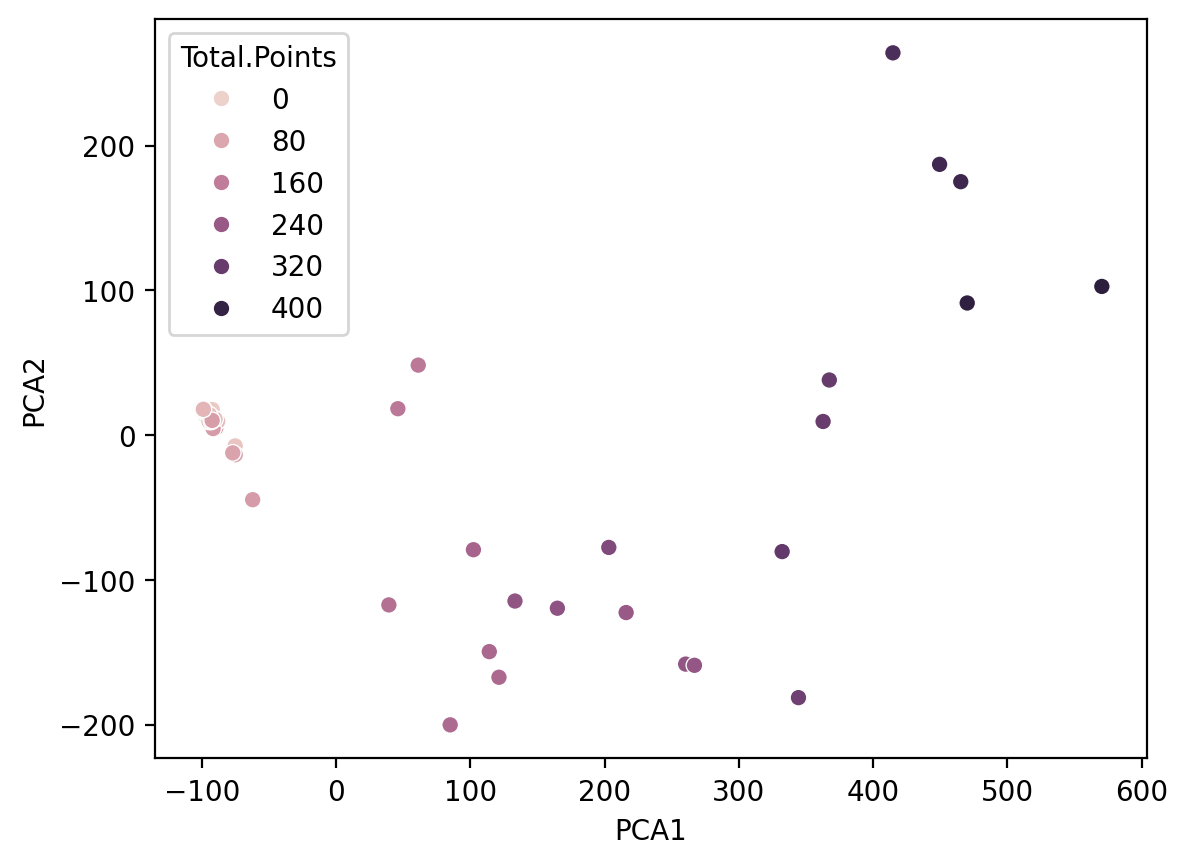
\includegraphics[width=\textwidth]{pca_plot.png}
    \caption{PCA Plot}
    \label{fig:pca}
\end{figure}

\begin{figure}[h!]
    \centering
    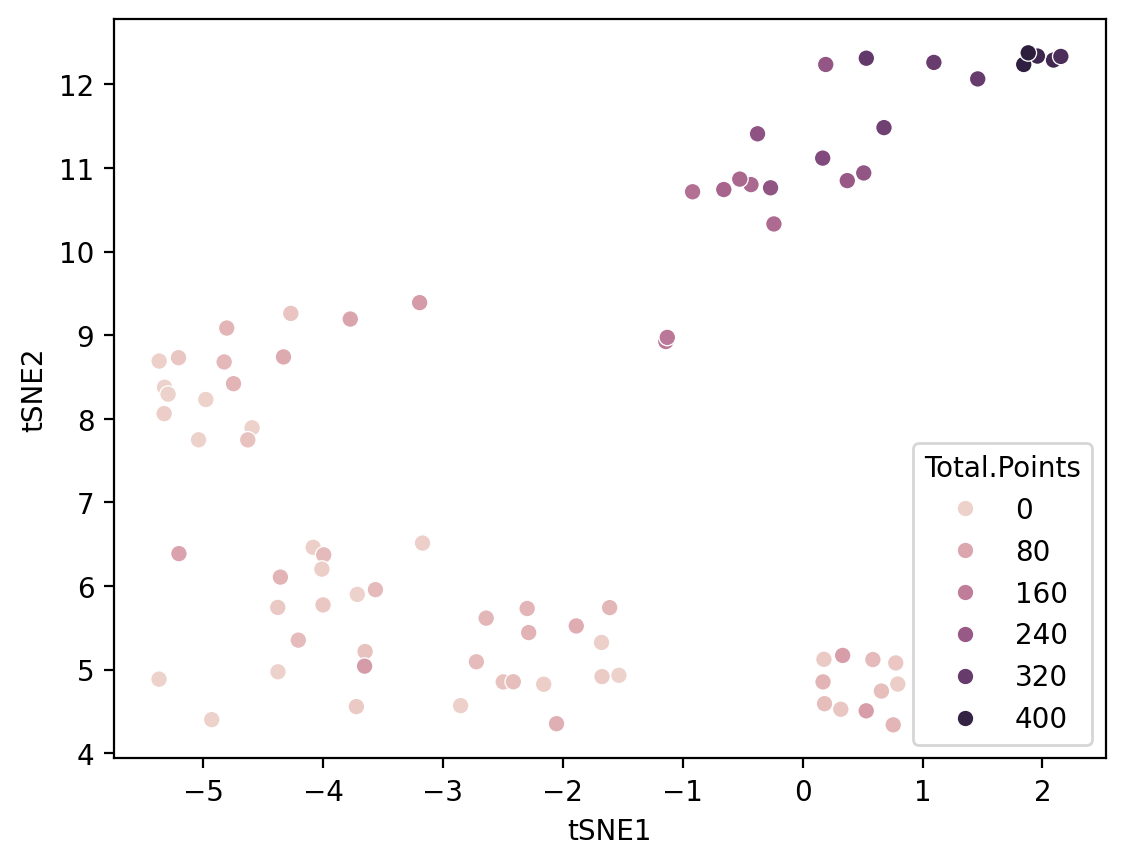
\includegraphics[width=\textwidth]{tsne_plot.png}
    \caption{t-SNE Plot}
    \label{fig:tsne}
\end{figure}

\subsection{Ταξινόμηση}
Η εφαρμογή υποστηρίζει δύο αλγορίθμους ταξινόμησης:
\begin{itemize}
    \item \textbf{Logistic Regression}: Εφαρμόζει λογιστική παλινδρόμηση για την ταξινόμηση των δεδομένων.
    \item \textbf{Random Forest Classifier}: Χρησιμοποιεί τυχαία δάση για την ταξινόμηση των δεδομένων.
\end{itemize}

\subsection{Ομαδοποίηση}
Διατίθενται δύο αλγόριθμοι ομαδοποίησης:
\begin{itemize}
    \item \textbf{KMeans}: Εκτελεί ομαδοποίηση χρησιμοποιώντας τον αλγόριθμο KMeans.
    \item \textbf{DBSCAN}: Εκτελεί ομαδοποίηση χρησιμοποιώντας τον αλγόριθμο DBSCAN.
\end{itemize}

\begin{figure}[h!]
    \centering
    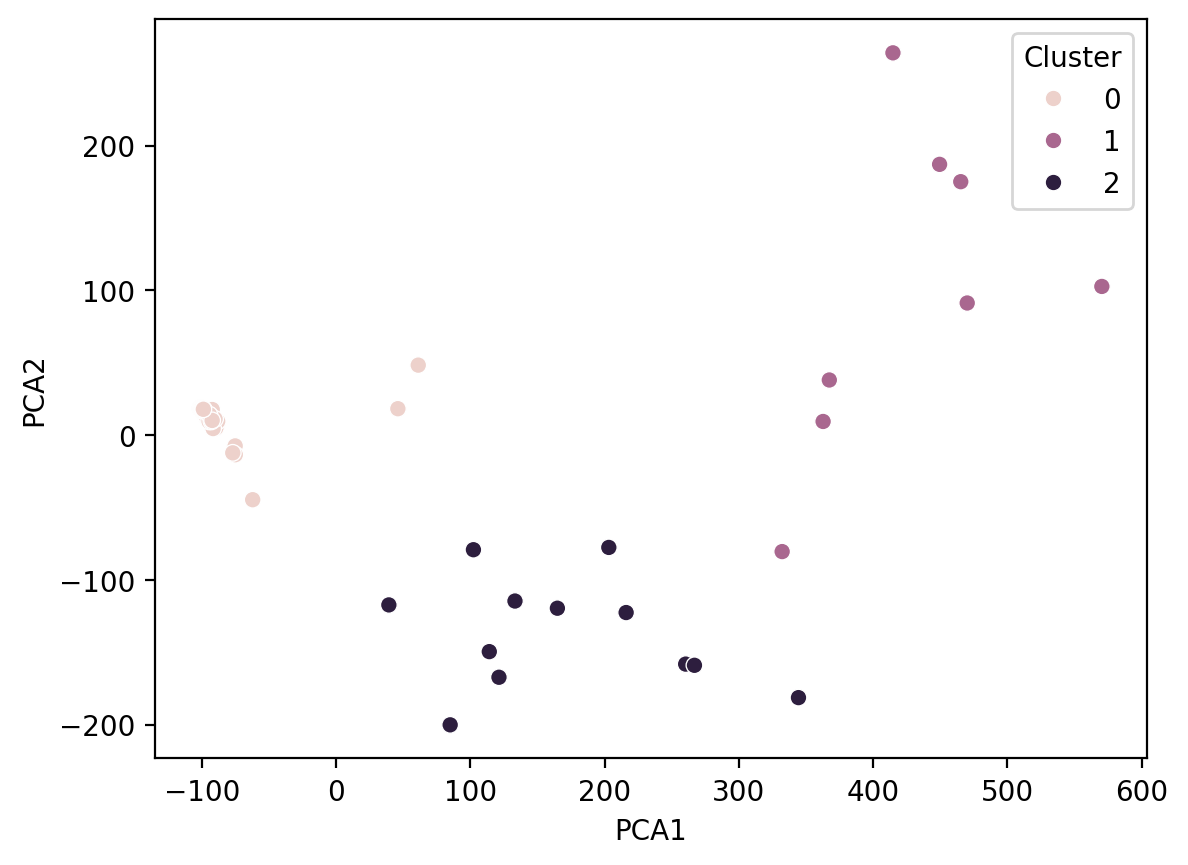
\includegraphics[width=\textwidth]{kmeans_plot.png}
    \caption{KMeans Plot}
    \label{fig:kmeans}
\end{figure}

\begin{figure}[h!]
    \centering
    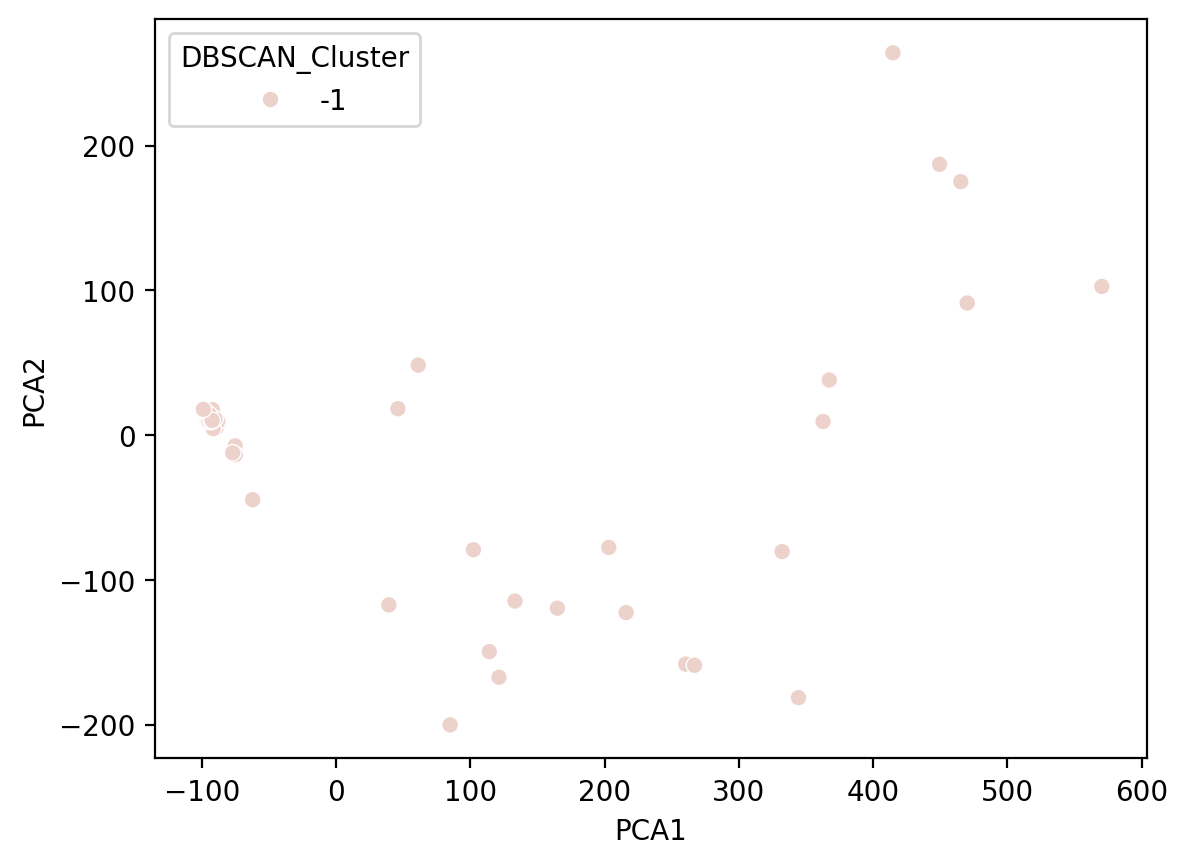
\includegraphics[width=\textwidth]{DBSCAN_CLUSTERING.PNG}
    \caption{DBSCAN Clustering}
    \label{fig:dbscan}
\end{figure}

\section{Οδηγίες Χρήσης}
\subsection{Οδηγίες Docker}
Για να δημιουργήσετε και να τρέξετε την εικόνα Docker της εφαρμογής:
\begin{itemize}
    \item \textbf{Δημιουργία εικόνας Docker}: \texttt{docker build -t data-analysis-sw .}
    \item \textbf{Εκτέλεση container Docker}: \texttt{docker run -p 8501:8501 my-streamlit-sw}
\end{itemize}

\subsection{Αποθετήριο GitHub}
Μπορείτε να βρείτε τον πηγαίο κώδικα και να συνεργαστείτε στο [GitHub](https://github.com/stamathsp/sw).

\section{Ομάδα Ανάπτυξης}
\begin{itemize}
    \item Παύλος - Μάριος Γιαννάκος
    \item Σταμάτης Πέτρου
\end{itemize}

\section{UML Διάγραμμα}
\begin{figure}[h]
    \centering
    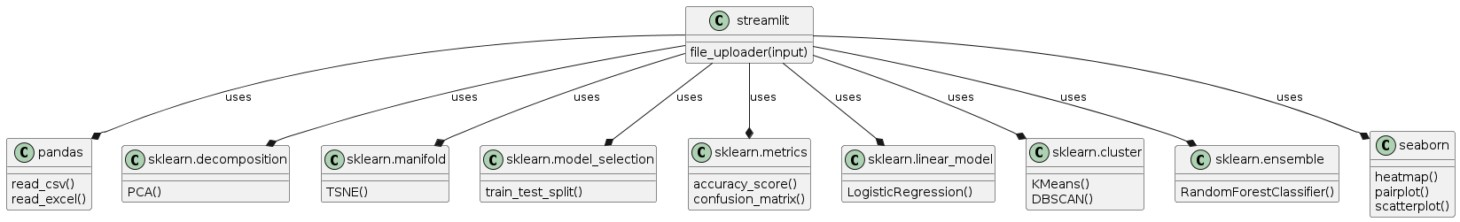
\includegraphics[width=\textwidth]{UML_diagram.jpg}
    \caption{UML Διάγραμμα της Εφαρμογής}
\end{figure}

\section{Στιγμιότυπα εφαρμογής}

\subsection{Στιγμιότυπο 94}
\begin{figure}[h!]
    \centering
    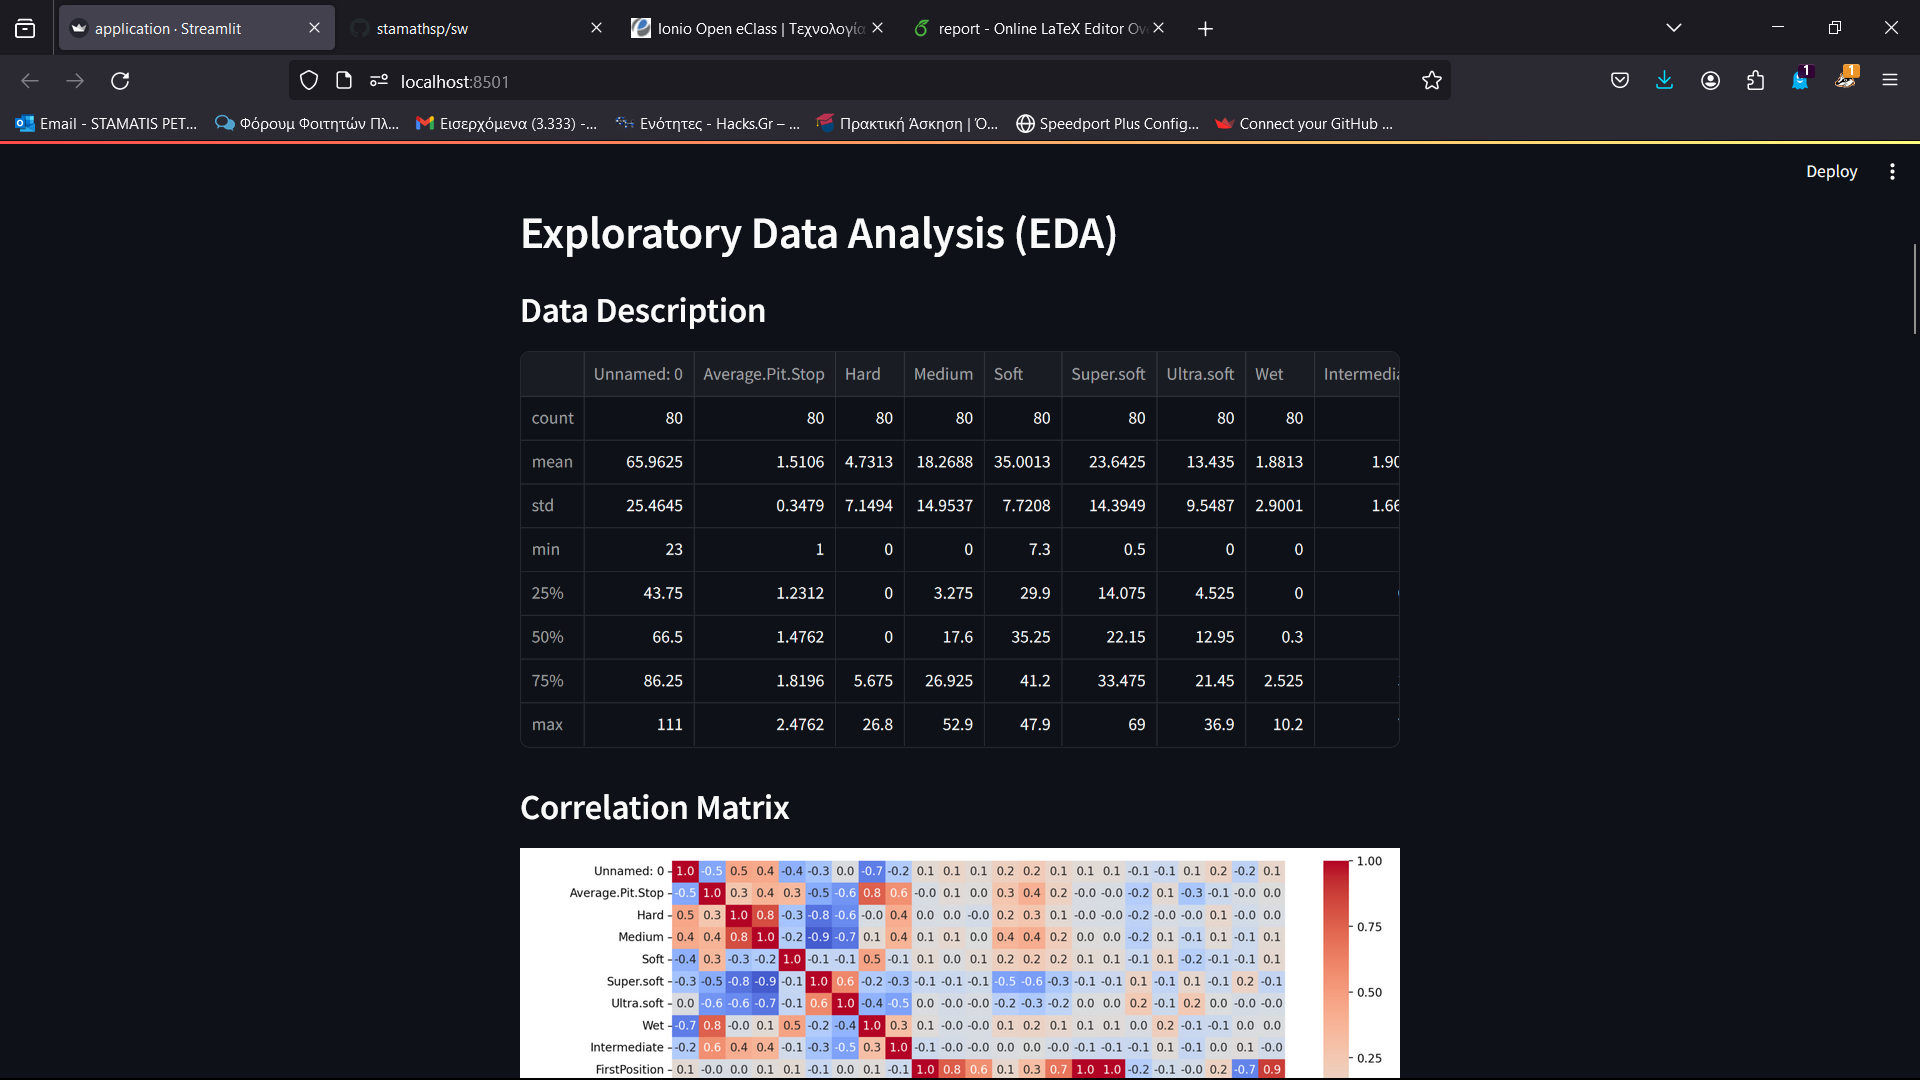
\includegraphics[width=\textwidth]{Screenshot (94).png}
    \caption{Στιγμιότυπο 94}
    \label{fig:screenshot94}
\end{figure}

\subsection{Στιγμιότυπο 95}
\begin{figure}[h!]
    \centering
    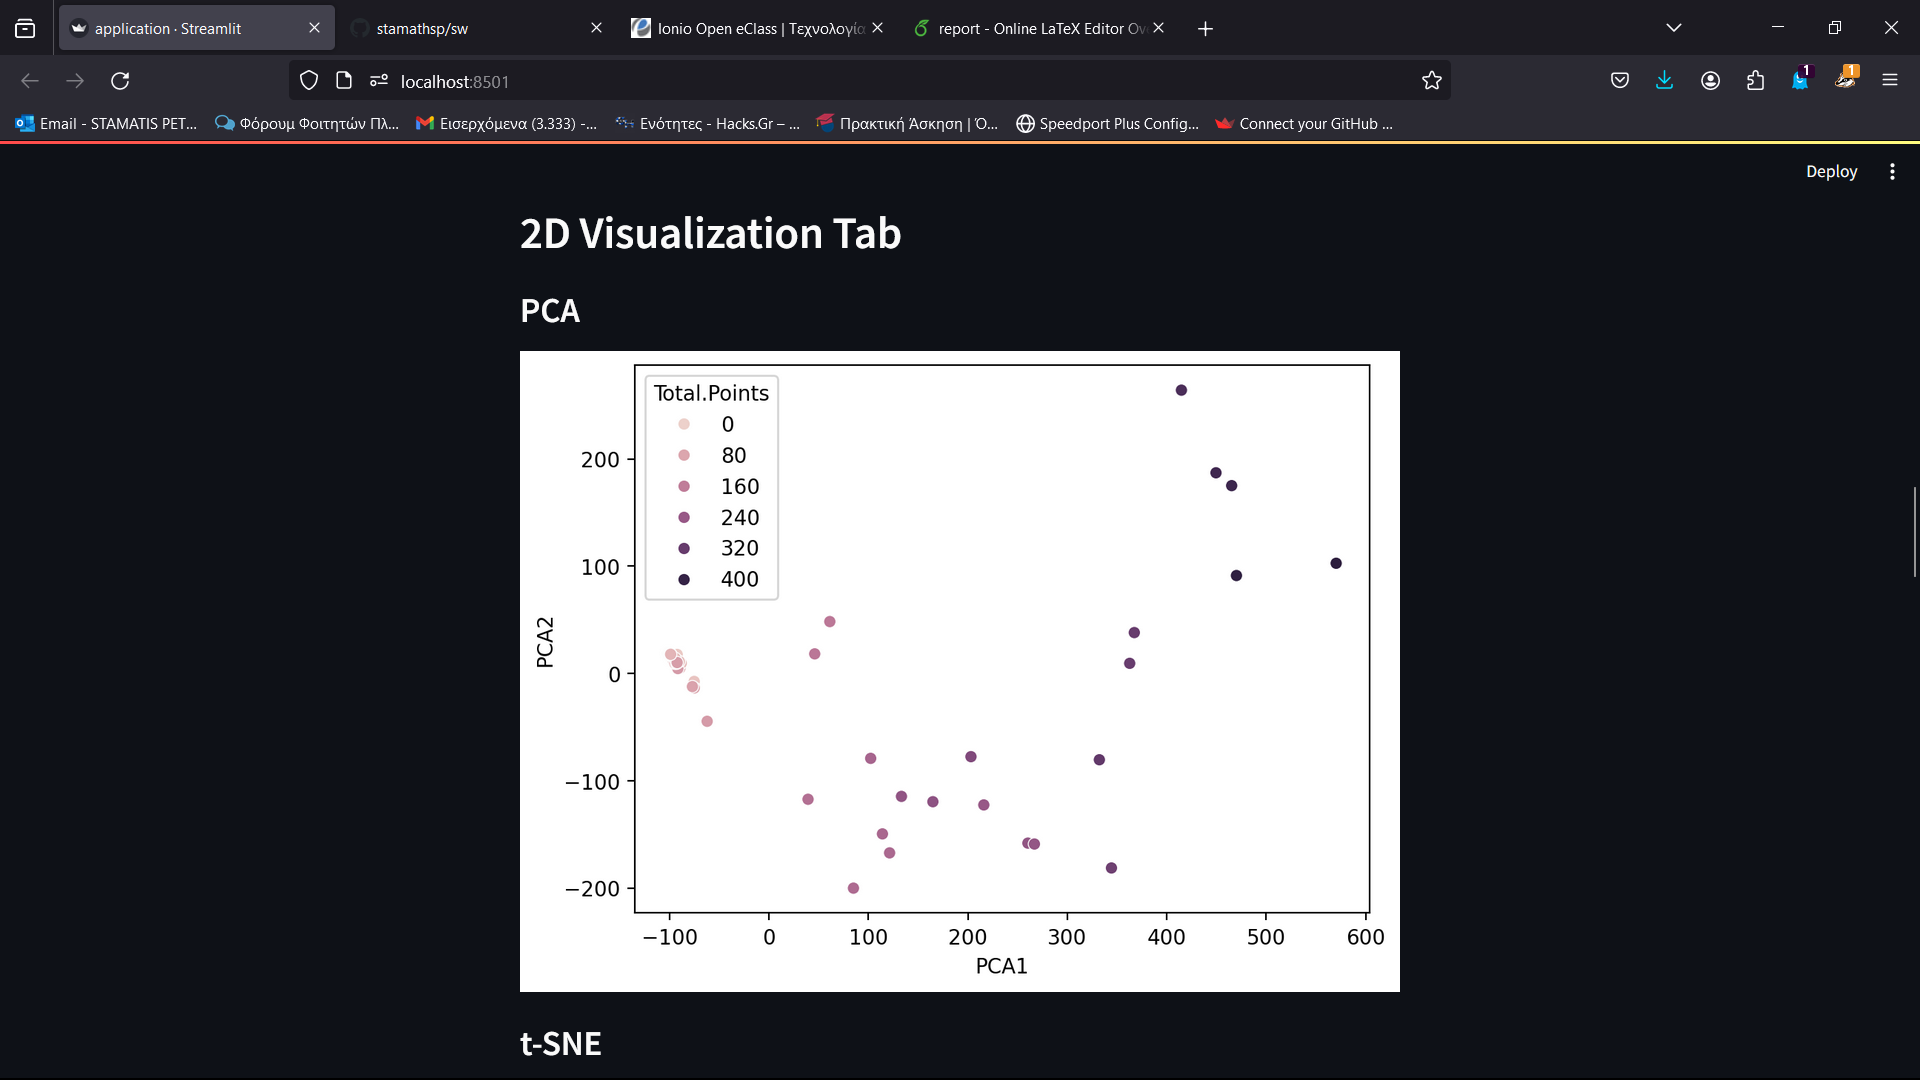
\includegraphics[width=\textwidth]{Screenshot (95).png}
    \caption{Στιγμιότυπο 95}
    \label{fig:screenshot95}
\end{figure}

\end{document}

